\documentclass[10pt,tgadventor, onlymath]{beamer}

\usepackage{graphicx,amsmath,amssymb,tikz,psfrag,neuralnetwork, fontawesome}

%\input defs.tex
\graphicspath{ {./figures/} }
\input defs.tex

%% formatting

\mode<presentation>
{
\usetheme{default}
\usetheme{Berlin}

\usecolortheme{seahorse}
}
\setbeamertemplate{navigation symbols}{}
\usecolortheme[rgb={0.03,0.28,0.59}]{structure}
\setbeamertemplate{itemize subitem}{--}
\setbeamertemplate{frametitle} {
	\begin{center}
	  {\large\bf \insertframetitle}
	\end{center}
}

\newcommand\footlineon{
  \setbeamertemplate{footline} {
    \begin{beamercolorbox}[ht=2.5ex,dp=1.125ex,leftskip=.8cm,rightskip=.6cm]{structure}
      \footnotesize \insertsection
      \hfill
      {\insertframenumber}
    \end{beamercolorbox}
    \vskip 0.45cm
  }
}
\footlineon

\AtBeginSection[] 
{ 
	\begin{frame}<beamer> 
		\frametitle{Outline} 
		\tableofcontents[currentsection,currentsubsection] 
	\end{frame} 
} 


\tikzstyle{state}=[shape=circle,draw=blue!30,fill=blue!10]
\tikzstyle{observation}=[shape=rectangle,draw=orange!30,fill=orange!10]
\tikzstyle{lightedge}=[<-, dashed]
\tikzstyle{mainstate}=[state, thick]
\tikzstyle{mainedge}=[<-, thick]
\tikzstyle{block} = [draw,rectangle,thick,minimum height=2em,minimum width=2em]
\tikzstyle{sum} = [draw,circle,inner sep=0mm,minimum size=2mm]
\tikzstyle{connector} = [->,thick]
\tikzstyle{line} = [thick]
\tikzstyle{branch} = [circle,inner sep=0pt,minimum size=1mm,fill=black,draw=black]
\tikzstyle{guide} = []
\tikzstyle{snakeline} = [connector, decorate, decoration={pre length=0.2cm,
                         post length=0.2cm, snake, amplitude=.4mm,
                         segment length=2mm},thick, magenta, ->]



%% begin presentation

\title{\large \bfseries Asymptotic Capacity of Systems with Intelligent Reflective Surface}

\author{Peter Hartig\\[3ex]}

\date{\today}

\begin{document}

\frame{
\thispagestyle{empty}
\titlepage
}

\section{Background}
\subsubsection{Devices}
\begin{frame}
\frametitle{Relaying}

	\begin{itemize}
		\item 			
			Relays vs. Base Stations (Not attached to core network? Why minimize this?)
		\item 
			Modes of operation provide cost/performance trade-off (decode and forward, amplify and forward ...)
		\item 
			Extending wireless coverage is relevant to high frequencies used in 5G +
	\end{itemize}
\end{frame}

\begin{frame}
\frametitle{Intelligent Reflective surface: Under the Hood}
\begin{columns}
\begin{column}{0.5\linewidth}
	Relay: Amplify and Forward
	\begin{equation*}
	\mathbf{y} = (\mathbf{H}_2\mathbf{F}\mathbf{H}_1 + \mathbf{G})\mathbf{x}
	\end{equation*}
	with $\mathbf{F}$ as the amplification factor
	\begin{itemize}
	\item 
		Can often ignore line of sight
	\item 
		Still requires expensive hardware
	\end{itemize}
\end{column}

\begin{column}{0.5\linewidth}
	IRS:
	\begin{equation*}
	\mathbf{y} = (\mathbf{H}_2\boldsymbol{\Phi}\mathbf{H}_1 + \mathbf{G})\mathbf{x}
	\end{equation*}
	with $\boldsymbol{\Phi}$ as diagonal matrix with elements $|\ \phi_i \| =1$.
	\begin{itemize}
	\item 
		No RF chain required (low cost)
	\item
		Shorter distances -> keep LOS
	\item 
		Current number of reflectors on models
	\end{itemize}
\end{column}
\end{columns}
\end{frame}


%\begin{frame}
%\frametitle{IRS: Modes of Operation}
%\begin{columns}
%\begin{column}{0.5\linewidth}
%	Mode 1
%	\begin{figure}
%%			\centering
%		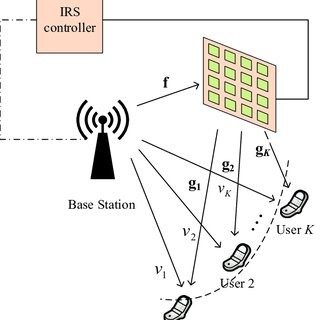
\includegraphics[scale=1]{irs}
%	\end{figure}\end{column}
%\begin{column}{0.5\linewidth}
%	Mode 2 (The one we will use)
%\end{column}
%\end{columns}
%\end{frame}
\begin{frame}
\frametitle{System Model}
\centering
\begin{equation}
	\mathbf{y} = (\mathbf{H}_2\boldsymbol{\Phi}\mathbf{H}_1 + \mathbf{G})\mathbf{x}
\end{equation}
with 
$\mathbf{H}_{1}\in \mathbb{C}_{S \times T},\mathbf{H}_{2} \in \mathbb{C}_{R \times S}, \mathbf{G} \in \mathbb{C}_{R \times T}$ and $\boldsymbol{\Phi}$ as diagonal matrix with elements $|\ \phi_i \| =1 $.
\end{frame}

\begin{frame}
\frametitle{Channel Capacity}
\begin{equation*}
	\mathbf{y} = (\mathbf{H}_2\boldsymbol{\Phi}\mathbf{H}_1 + \mathbf{G})\mathbf{x}
\end{equation*}

Capacity is given by 
\begin{equation}\label{capacity}
\underset{\mathbf{Q}_{x}, \boldsymbol{\Phi} }{\mathrm{max}}
\Expect\left[\Log\left(|\mathbf{I}_{N_R}+\frac{1}{\sigma_n}[\mathbf{H}_{2}\boldsymbol{\Phi}\mathbf{H}_{1} + \mathbf{G}]\mathbf{Q}_x[\mathbf{H}_{2}\boldsymbol{\Phi}\mathbf{H}_{1} + \mathbf{G}]^H|\right)\right].
\end{equation}
Using 
\begin{equation}
\mathbf{H}_{\text{Total}} = \mathbf{H}_{2}\boldsymbol{\Phi}\mathbf{H}_{1} + \mathbf{G}
\end{equation}
and simplifying, \ref{capacity} becomes
\begin{equation}
\underset{\mathbf{Q}_{x}, \boldsymbol{\Phi} }{\mathrm{max}}
N\Expect\left[\Log\left(1+\frac{1}{\sigma_n} + \lambda\right)\right]
\end{equation}
Need Asymptotic Eigenvalue Distribution $p(\lambda)$ (AED) to evaluate the expectation.
\end{frame}


\subsubsection{Previous Work + Free Probability}
\begin{frame}
\frametitle{Free Probability}
Introduce the SVD AED relationship.
\end{frame}

\begin{frame}
\frametitle{Free Probability}
Show how to solve for individual covariance matrices and point out that phases cancel.
Asymptotic analysis
\end{frame}


\section{Goals}
\begin{frame}
\frametitle{Project Goals}
\begin{enumerate}
\item
	Find capacity of asymptotic IRS systems
\item
	Extend results to secrecy capacity
\item 
	Confirm findings with numerical results throughout
\end{enumerate}
\end{frame}

\section{Current Status}
\begin{frame}
\frametitle{Current Status}
\begin{enumerate}
\item
	Find capacity of asymptotic IRS systems: \faCheck
\item
	Extend results to secrecy capacity: TODO
\item 
	Confirm findings with numerical results throughout
\end{enumerate}

\end{frame}


\section{Conclusion}

\begin{frame}
  \centering \Large
  \emph{Thank You.}
  \\
	\bigskip
    \centering \Large
  \emph{Questions or Comments?}

\end{frame}





\end{document}
